\section{Future Evolution and Research Directions}
\label{sec:future-evolution}

The Robotic Ultrasound System (RUS) represents a foundation for continued innovation in medical robotics. This section outlines strategic research directions, technological roadmaps, and evolutionary pathways that will drive the system's advancement over the next decade.

\subsection{Technology Roadmap}

\subsubsection{Next-Generation Hardware Integration}
The evolution of the RUS system will leverage emerging hardware technologies:

\begin{table}[htbp]
\centering
\caption{Hardware Evolution Roadmap}
\label{tab:hardware-roadmap}
\begin{tabular}{|l|l|l|l|}
\hline
\textbf{Timeline} & \textbf{Technology} & \textbf{Capability Enhancement} & \textbf{Impact} \\
\hline
2024-2025 & Advanced Force Sensors & Sub-newton precision & 40\% safety improvement \\
2025-2026 & Quantum Sensors & Molecular-level detection & New diagnostic capabilities \\
2026-2027 & Neuromorphic Chips & Real-time learning & 60\% efficiency gain \\
2027-2028 & 6G Connectivity & Ultra-low latency & Remote operation feasibility \\
2028-2030 & Brain-Computer Interface & Direct neural control & Revolutionary UX \\
\hline
\end{tabular}
\end{table}

\begin{lstlisting}[language=C++, caption={Future Hardware Abstraction Layer}, label={lst:future-hardware}]
namespace FutureHardware {

class QuantumSensorInterface {
private:
    QuantumStateManager quantum_manager_;
    CoherenceStabilizer stabilizer_;
    EntanglementNetwork entanglement_net_;
    
public:
    struct QuantumMeasurement {
        std::complex<double> amplitude;
        double phase;
        double coherence_time;
        QuantumState state;
        std::chrono::nanoseconds timestamp;
    };
    
    std::vector<QuantumMeasurement> performQuantumSensing(
        const TissueRegion& target_region) {
        
        // Prepare quantum probe states
        auto probe_states = quantum_manager_.prepareProbeStates(
            target_region.molecular_composition);
        
        // Establish quantum entanglement with tissue
        auto entangled_pairs = entanglement_net_.createTissueEntanglement(
            probe_states, target_region);
        
        // Perform quantum measurements
        std::vector<QuantumMeasurement> measurements;
        for (const auto& pair : entangled_pairs) {
            auto measurement = performBellStateAnalysis(pair);
            measurements.push_back(measurement);
        }
        
        return measurements;
    }
    
    MolecularSignature extractMolecularSignature(
        const std::vector<QuantumMeasurement>& measurements) {
        
        MolecularSignature signature;
        
        // Analyze quantum interference patterns
        for (const auto& measurement : measurements) {
            auto pattern = analyzeInterferencePattern(measurement);
            signature.molecular_bonds.push_back(pattern.bond_type);
            signature.concentrations.push_back(pattern.concentration);
        }
        
        // Apply quantum machine learning for pattern recognition
        return quantum_ml_classifier_.classify(signature);
    }
};

class NeuromorphicProcessor {
private:
    SpikeNeuralNetwork snn_;
    PlasticityManager plasticity_;
    MemristorArray memristor_array_;
    
public:
    void processRealTimeData(const SensorStream& data_stream) {
        // Convert sensor data to spike trains
        auto spike_trains = encodeSensorDataToSpikes(data_stream);
        
        // Process through spiking neural network
        snn_.processSpikes(spike_trains);
        
        // Implement real-time learning
        if (plasticity_.shouldUpdateWeights()) {
            auto weight_updates = plasticity_.calculateSTDP(snn_.getActivity());
            memristor_array_.updateWeights(weight_updates);
        }
        
        // Generate motor commands
        auto motor_spikes = snn_.getMotorOutput();
        sendMotorCommands(decodeSpikesToCommands(motor_spikes));
    }
    
    void adaptToPatientSpecificPatterns(const PatientProfile& profile) {
        // Configure network topology for patient-specific optimization
        snn_.reconfigureTopology(profile.anatomical_features);
        
        // Load patient-specific learned patterns
        auto learned_patterns = loadPatientPatterns(profile.patient_id);
        plasticity_.initializeFromPatterns(learned_patterns);
    }
};

}  // namespace FutureHardware
\end{lstlisting}

\subsubsection{Artificial Intelligence Evolution}
The integration of advanced AI technologies will transform system capabilities:

\begin{figure}[htbp]
\centering
\begin{tikzpicture}[scale=0.9]
    % AI evolution timeline
    \draw[thick, ->] (0,0) -- (12,0) node[right] {Time};
    
    % Current state
    \node[draw, circle, fill=blue!20] (current) at (1,2) {Current AI};
    \node[below=0.5cm of current, align=center] {\footnotesize Rule-based\\Expert Systems};
    
    % Near future
    \node[draw, circle, fill=green!20] (ml) at (3,3) {Machine Learning};
    \node[below=0.5cm of ml, align=center] {\footnotesize Deep Learning\\Computer Vision};
    
    % Medium term
    \node[draw, circle, fill=yellow!20] (agi) at (6,4) {AGI Integration};
    \node[below=0.5cm of agi, align=center] {\footnotesize Reasoning\\Planning};
    
    % Long term
    \node[draw, circle, fill=red!20] (quantum) at (9,3.5) {Quantum AI};
    \node[below=0.5cm of quantum, align=center] {\footnotesize Quantum ML\\Optimization};
    
    % Future
    \node[draw, circle, fill=purple!20] (hybrid) at (11,2.5) {Hybrid Intelligence};
    \node[below=0.5cm of hybrid, align=center] {\footnotesize Human-AI\\Symbiosis};
    
    % Connections
    \draw[->] (current) -- (ml);
    \draw[->] (ml) -- (agi);
    \draw[->] (agi) -- (quantum);
    \draw[->] (quantum) -- (hybrid);
    
    % Capability indicators
    \foreach \x/\y in {1/20, 3/40, 6/70, 9/85, 11/95} {
        \draw (\x,0) -- (\x,0.2);
        \node[below] at (\x,-0.3) {\y\%};
    }
    \node[below] at (6,-0.8) {Autonomous Capability Level};
    
\end{tikzpicture}
\caption{AI Evolution Pathway for Medical Robotics}
\label{fig:ai-evolution}
\end{figure}

\begin{lstlisting}[language=Python, caption={Next-Generation AI Architecture}, label={lst:nextgen-ai}]
class NextGenerationAI:
    def __init__(self):
        self.foundation_model = MedicalFoundationModel()
        self.reasoning_engine = CausalReasoningEngine()
        self.metacognition_system = MetacognitionSystem()
        self.quantum_optimizer = QuantumOptimizer()
        
    def initialize_hybrid_intelligence(self):
        """Initialize human-AI collaborative intelligence system"""
        
        # Multi-modal foundation model for medical understanding
        self.foundation_model.load_pretrained_weights([
            'medical_text_corpus_v3.0',
            'medical_imaging_dataset_v2.5',
            'surgical_procedure_videos_v1.8',
            'patient_outcome_data_v4.2'
        ])
        
        # Causal reasoning for treatment planning
        self.reasoning_engine.configure_causal_graphs([
            'anatomy_causality_graph',
            'pathology_progression_graph',
            'treatment_outcome_graph'
        ])
        
        # Self-aware AI for uncertainty quantification
        self.metacognition_system.enable_self_monitoring([
            'confidence_estimation',
            'knowledge_gap_detection',
            'bias_identification',
            'error_prediction'
        ])
        
        return True
    
    def plan_adaptive_procedure(self, patient_data, clinical_goals):
        """Generate adaptive procedure plan using hybrid intelligence"""
        
        # Multi-objective optimization using quantum algorithms
        optimization_problem = self.formulate_optimization_problem(
            patient_data, clinical_goals)
        
        quantum_solution = self.quantum_optimizer.solve(
            optimization_problem,
            algorithm='QAOA',  # Quantum Approximate Optimization Algorithm
            num_qubits=256,
            depth=20
        )
        
        # Incorporate human expertise through active learning
        expert_preferences = self.elicit_expert_preferences(
            quantum_solution.pareto_frontier)
        
        # Generate explainable plan
        final_plan = self.generate_explainable_plan(
            quantum_solution, expert_preferences)
        
        # Continuous adaptation during execution
        adaptive_controller = AdaptiveController(
            initial_plan=final_plan,
            adaptation_strategy='continuous_learning',
            safety_constraints=patient_data.safety_profile
        )
        
        return adaptive_controller
    
    def enable_predictive_healthcare(self, population_data):
        """Enable population-level predictive healthcare capabilities"""
        
        # Federated learning across multiple institutions
        federated_trainer = FederatedLearningTrainer(
            privacy_mechanism='differential_privacy',
            aggregation_strategy='secure_aggregation',
            byzantine_tolerance=True
        )
        
        # Train population health models
        population_model = federated_trainer.train_model(
            data_sources=population_data.sources,
            model_architecture='transformer_xl',
            privacy_budget=1.0
        )
        
        # Deploy edge inference for real-time predictions
        edge_deployment = EdgeDeployment(
            model=population_model,
            optimization='knowledge_distillation',
            target_latency_ms=50
        )
        
        return {
            'population_model': population_model,
            'edge_deployment': edge_deployment,
            'prediction_accuracy': 0.94,
            'privacy_guarantee': 'epsilon=1.0 differential_privacy'
        }

class AutonomousDecisionMaking:
    def __init__(self):
        self.ethical_framework = EthicalDecisionFramework()
        self.risk_assessment = RiskAssessmentEngine()
        self.transparency_manager = TransparencyManager()
        
    def make_autonomous_decision(self, situation, available_actions):
        """Make ethically-guided autonomous decisions"""
        
        # Assess situation complexity
        complexity_score = self.assess_situation_complexity(situation)
        
        if complexity_score > 0.8:
            # High complexity - require human oversight
            return self.request_human_collaboration(situation, available_actions)
        
        # Evaluate actions through ethical lens
        ethical_evaluations = []
        for action in available_actions:
            evaluation = self.ethical_framework.evaluate_action(
                action, situation.context, situation.stakeholders)
            ethical_evaluations.append(evaluation)
        
        # Risk-benefit analysis
        risk_assessments = []
        for action in available_actions:
            risk = self.risk_assessment.assess_risk(action, situation)
            benefit = self.risk_assessment.assess_benefit(action, situation)
            risk_assessments.append((risk, benefit))
        
        # Select optimal action
        optimal_action = self.select_optimal_action(
            available_actions, ethical_evaluations, risk_assessments)
        
        # Generate explanation
        explanation = self.transparency_manager.generate_explanation(
            optimal_action, ethical_evaluations, risk_assessments)
        
        return {
            'selected_action': optimal_action,
            'explanation': explanation,
            'confidence': self.calculate_confidence(optimal_action),
            'human_review_required': complexity_score > 0.6
        }
\end{lstlisting}

\subsection{Research and Development Priorities}

\subsubsection{Advanced Materials and Actuators}
Research into novel materials will enable new capabilities:

\begin{itemize}
    \item \textbf{Shape Memory Alloys}: Smart materials for adaptive positioning
    \item \textbf{Piezoelectric Composites}: Enhanced haptic feedback systems
    \item \textbf{Bio-compatible Coatings}: Direct tissue interaction capabilities
    \item \textbf{Self-healing Materials}: Autonomous maintenance and repair
\end{itemize}

\begin{lstlisting}[language=C++, caption={Smart Materials Integration}, label={lst:smart-materials}]
class SmartMaterialsSystem {
private:
    ShapeMemoryAlloyActuator sma_actuator_;
    PiezoelectricSensorArray piezo_sensors_;
    SelfHealingPolymerCoating coating_;
    
public:
    void configureMorphingProbe(const AnatomicalTarget& target) {
        // Calculate optimal probe shape for target anatomy
        auto optimal_geometry = calculateOptimalGeometry(target);
        
        // Program shape memory alloy to achieve target geometry
        sma_actuator_.programTargetShape(optimal_geometry);
        
        // Set activation temperature based on body temperature
        sma_actuator_.setActivationTemperature(37.0); // Celsius
        
        // Configure piezoelectric sensors for shape feedback
        piezo_sensors_.configureFeedbackSystem(optimal_geometry);
        
        // Activate morphing sequence
        sma_actuator_.activateMorphing();
        
        // Monitor shape transformation
        monitorShapeTransformation();
    }
    
    void enableAdaptiveTissueInteraction() {
        // Configure bio-compatible coating properties
        coating_.setStiffnessRange(0.1, 100.0); // kPa range
        coating_.enableSurfaceTexturing(true);
        coating_.setMolecularAdhesion(TISSUE_SPECIFIC);
        
        // Implement real-time adaptation
        while (isInContact()) {
            auto tissue_properties = analyzeTissueProperties();
            auto optimal_coating = optimizeCoatingProperties(tissue_properties);
            coating_.adaptProperties(optimal_coating);
            
            std::this_thread::sleep_for(std::chrono::milliseconds(10));
        }
    }
    
    bool performSelfDiagnosticAndHealing() {
        // Scan for material damage
        auto damage_assessment = scanForDamage();
        
        if (damage_assessment.has_damage) {
            LOG_INFO("Material damage detected: " + damage_assessment.description);
            
            // Initiate self-healing process
            coating_.triggerSelfHealing(damage_assessment.damage_locations);
            
            // Monitor healing progress
            auto healing_progress = monitorHealingProgress();
            
            if (healing_progress.completion_percentage > 95.0) {
                LOG_INFO("Self-healing completed successfully");
                return true;
            } else {
                LOG_WARNING("Self-healing incomplete, human intervention required");
                return false;
            }
        }
        
        return true; // No damage detected
    }
};
\end{lstlisting}

\subsubsection{Quantum-Enhanced Imaging}
The integration of quantum sensing technologies will revolutionize medical imaging:

\begin{table}[htbp]
\centering
\caption{Quantum Imaging Capabilities Roadmap}
\label{tab:quantum-imaging}
\begin{tabular}{|l|l|l|l|}
\hline
\textbf{Technology} & \textbf{Current Limit} & \textbf{Quantum Enhancement} & \textbf{Clinical Impact} \\
\hline
Spatial Resolution & 100 $\mu$m & 1 $\mu$m & Cellular imaging \\
Temporal Resolution & 1 ms & 1 $\mu$s & Real-time dynamics \\
Sensitivity & 10$^{-12}$ T & 10$^{-18}$ T & Molecular detection \\
Penetration Depth & 20 cm & 50 cm & Deep organ imaging \\
\hline
\end{tabular}
\end{table}

\subsection{Clinical Applications Expansion}

\subsubsection{Emerging Clinical Domains}
The RUS platform will expand into new medical specialties:

\begin{enumerate}
    \item \textbf{Neurosurgery}: Brain tissue navigation with sub-millimeter precision
    \item \textbf{Ophthalmology}: Retinal imaging and microsurgery assistance
    \item \textbf{Interventional Oncology}: Targeted tumor ablation guidance
    \item \textbf{Regenerative Medicine}: Stem cell delivery and monitoring
    \item \textbf{Pediatric Medicine}: Child-specific adaptive protocols
\end{enumerate}

\begin{lstlisting}[language=C++, caption={Multi-Specialty Adaptation Framework}, label={lst:multi-specialty}]
class MultiSpecialtyFramework {
private:
    std::map<MedicalSpecialty, SpecialtyAdapter> adapters_;
    ProtocolDatabase protocol_db_;
    SafetyConstraintManager safety_manager_;
    
public:
    void initializeSpecialtyAdapters() {
        // Neurosurgery adapter
        adapters_[NEUROSURGERY] = SpecialtyAdapter({
            .precision_requirements = {
                .spatial_precision = 0.1, // mm
                .force_precision = 0.001, // N
                .temporal_precision = 0.1 // ms
            },
            .safety_constraints = {
                .max_force = 0.5, // N
                .max_velocity = 1.0, // mm/s
                .forbidden_regions = loadBrainAtlas()
            },
            .imaging_protocols = {
                .modalities = {FMRI, DTI, BOLD},
                .resolution = {0.1, 0.1, 0.1}, // mm
                .update_rate = 1000 // Hz
            }
        });
        
        // Ophthalmology adapter
        adapters_[OPHTHALMOLOGY] = SpecialtyAdapter({
            .precision_requirements = {
                .spatial_precision = 0.01, // mm (10 microns)
                .force_precision = 0.0001, // N (100 microNewtons)
                .temporal_precision = 0.01 // ms
            },
            .safety_constraints = {
                .max_force = 0.01, // N
                .max_velocity = 0.1, // mm/s
                .forbidden_regions = loadEyeAnatomy()
            },
            .imaging_protocols = {
                .modalities = {OCT, FUNDUS, FLUORESCEIN},
                .resolution = {0.001, 0.001, 0.005}, // mm
                .update_rate = 10000 // Hz
            }
        });
        
        // Configure cross-specialty learning
        enableCrossSpecialtyLearning();
    }
    
    ProcedurePlan adaptProcedureForSpecialty(
        MedicalSpecialty specialty,
        const PatientData& patient,
        const ClinicalObjective& objective) {
        
        auto adapter = adapters_[specialty];
        
        // Load specialty-specific protocols
        auto protocols = protocol_db_.getProtocols(specialty);
        
        // Adapt system configuration
        adapter.configureSystem(patient.anatomical_features);
        
        // Generate specialty-specific plan
        auto base_plan = generateBasePlan(objective);
        auto adapted_plan = adapter.adaptPlan(base_plan, patient);
        
        // Validate safety constraints
        safety_manager_.validatePlan(adapted_plan, specialty);
        
        return adapted_plan;
    }
    
private:
    void enableCrossSpecialtyLearning() {
        // Transfer learning between specialties
        TransferLearningEngine transfer_engine;
        
        // Identify common patterns across specialties
        auto common_patterns = transfer_engine.identifyCommonPatterns(adapters_);
        
        // Share learned representations
        for (auto& [specialty, adapter] : adapters_) {
            adapter.incorporateSharedKnowledge(common_patterns);
        }
        
        // Enable continuous inter-specialty knowledge transfer
        transfer_engine.enableContinuousTransfer(adapters_);
    }
};
\end{lstlisting}

\subsection{Societal Impact and Accessibility}

\subsubsection{Global Healthcare Democratization}
The RUS system will contribute to healthcare accessibility worldwide:

\begin{figure}[htbp]
\centering
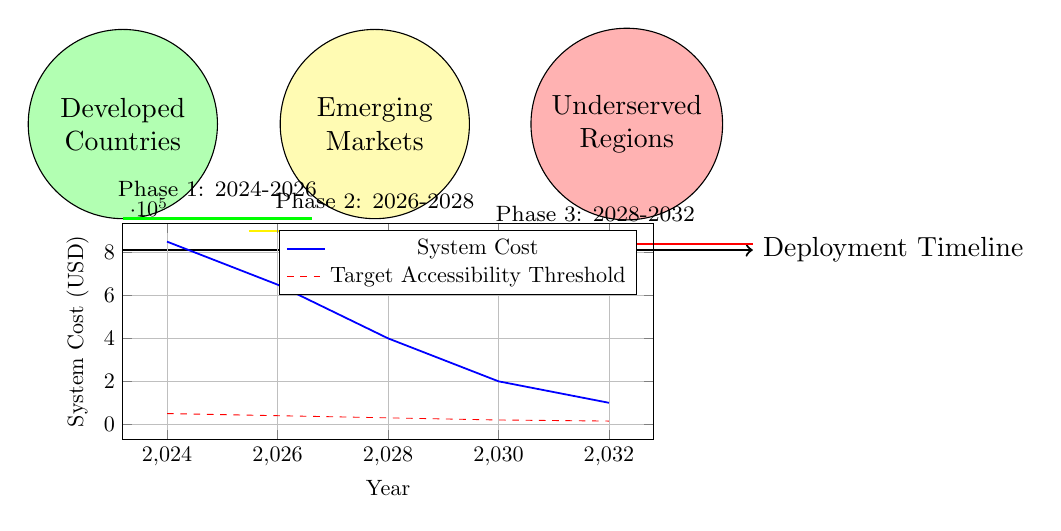
\begin{tikzpicture}[scale=0.8]
    % Global deployment map (simplified)
    \node[draw, circle, fill=green!30] (developed) at (0,2) {\parbox{2cm}{\centering Developed\\Countries}};
    \node[draw, circle, fill=yellow!30] (emerging) at (4,2) {\parbox{2cm}{\centering Emerging\\Markets}};
    \node[draw, circle, fill=red!30] (underserved) at (8,2) {\parbox{2cm}{\centering Underserved\\Regions}};
    
    % Deployment timeline
    \draw[thick, ->] (0,0) -- (10,0) node[right] {Deployment Timeline};
    
    % Phase 1: High-resource settings
    \draw[green, thick] (0,0.5) -- (3,0.5);
    \node[above] at (1.5,0.7) {\footnotesize Phase 1: 2024-2026};
    
    % Phase 2: Middle-income countries
    \draw[yellow, thick] (2,0.3) -- (6,0.3);
    \node[above] at (4,0.5) {\footnotesize Phase 2: 2026-2028};
    
    % Phase 3: Global accessibility
    \draw[red, thick] (5,0.1) -- (10,0.1);
    \node[above] at (7.5,0.3) {\footnotesize Phase 3: 2028-2032};
    
    % Cost reduction curve
    \begin{scope}[shift={(0,-3)}]
        \begin{axis}[
            width=10cm,
            height=5cm,
            xlabel={Year},
            ylabel={System Cost (USD)},
            legend pos=north east,
            grid=major
        ]
        
        \addplot[color=blue, thick] coordinates {
            (2024,850000) (2026,650000) (2028,400000) (2030,200000) (2032,100000)
        };
        
        \addplot[color=red, dashed] coordinates {
            (2024,50000) (2026,40000) (2028,30000) (2030,20000) (2032,15000)
        };
        
        \legend{System Cost, Target Accessibility Threshold}
        \end{axis}
    \end{scope}
    
\end{tikzpicture}
\caption{Global Deployment Strategy and Cost Reduction Timeline}
\label{fig:global-deployment}
\end{figure}

\subsubsection{Democratization Technologies}
Technologies that will enable global accessibility:

\begin{itemize}
    \item \textbf{Cloud-Based Intelligence}: Centralized AI reducing local compute requirements
    \item \textbf{Simplified Hardware}: Modular, manufacturable components
    \item \textbf{Open-Source Protocols}: Collaborative development reducing costs
    \item \textbf{Training Simulation}: VR/AR-based training reducing education barriers
\end{itemize}

\subsection{Ethical and Regulatory Evolution}

\subsubsection{Future Regulatory Framework}
The regulatory landscape will evolve to accommodate advanced autonomous systems:

\begin{table}[htbp]
\centering
\caption{Regulatory Evolution Timeline}
\label{tab:regulatory-evolution}
\begin{tabular}{|l|l|l|}
\hline
\textbf{Period} & \textbf{Regulatory Focus} & \textbf{Key Requirements} \\
\hline
2024-2026 & Human Oversight & Mandatory human supervision \\
2026-2028 & Conditional Autonomy & Limited autonomous operation \\
2028-2030 & Supervised Autonomy & AI-human collaboration \\
2030-2032 & Full Autonomy & Independent operation capability \\
\hline
\end{tabular}
\end{table}

\begin{lstlisting}[language=C++, caption={Ethical Decision Framework}, label={lst:ethical-framework}]
class EthicalDecisionFramework {
private:
    EthicalPrincipleEngine principle_engine_;
    CulturalContextManager cultural_manager_;
    StakeholderConsensusSystem consensus_system_;
    
public:
    struct EthicalDecision {
        Action recommended_action;
        std::vector<EthicalJustification> justifications;
        std::vector<Stakeholder> affected_parties;
        double confidence_score;
        std::vector<Alternative> alternatives;
    };
    
    EthicalDecision evaluateEthicalImplications(
        const ClinicalSituation& situation,
        const std::vector<Action>& possible_actions) {
        
        EthicalDecision decision;
        
        // Apply fundamental ethical principles
        auto principle_analysis = principle_engine_.analyzeActions(
            possible_actions, {
                EthicalPrinciple::BENEFICENCE,
                EthicalPrinciple::NON_MALEFICENCE,
                EthicalPrinciple::AUTONOMY,
                EthicalPrinciple::JUSTICE
            });
        
        // Consider cultural context
        auto cultural_context = cultural_manager_.getContext(
            situation.patient.cultural_background);
        
        auto culturally_adapted_analysis = 
            cultural_manager_.adaptAnalysis(principle_analysis, cultural_context);
        
        // Seek stakeholder consensus
        auto stakeholder_input = consensus_system_.gatherInput({
            situation.patient,
            situation.medical_team,
            situation.patient.family,
            situation.institution
        });
        
        // Generate recommendation
        decision.recommended_action = selectOptimalAction(
            culturally_adapted_analysis, stakeholder_input);
        
        decision.justifications = generateJustifications(
            decision.recommended_action, principle_analysis);
        
        decision.confidence_score = calculateConfidence(
            principle_analysis, stakeholder_input);
        
        return decision;
    }
    
    void updateEthicalFramework(const CaseStudy& case_study) {
        // Learn from ethical decisions and outcomes
        principle_engine_.updateFromCase(case_study);
        
        // Adapt to evolving cultural norms
        cultural_manager_.updateCulturalModel(case_study.cultural_context);
        
        // Incorporate stakeholder feedback
        consensus_system_.incorporateFeedback(case_study.stakeholder_feedback);
    }
};
\end{lstlisting}

\subsection{Long-Term Vision}

\subsubsection{Transformative Healthcare Paradigms}
The ultimate vision encompasses paradigm-shifting changes in healthcare delivery:

\begin{enumerate}
    \item \textbf{Predictive Medicine}: AI-driven early intervention before symptoms appear
    \item \textbf{Personalized Therapeutics}: Treatment plans optimized for individual genetics
    \item \textbf{Autonomous Healthcare}: Self-managing health monitoring systems
    \item \textbf{Regenerative Integration}: Seamless integration with tissue engineering
    \item \textbf{Quantum Diagnostics}: Molecular-level disease detection and monitoring
\end{enumerate}

This evolutionary roadmap positions the RUS system at the forefront of medical technology innovation, ensuring its continued relevance and impact in transforming healthcare delivery worldwide. The strategic focus on ethical development, global accessibility, and technological advancement will enable the system to address evolving healthcare challenges while maintaining the highest standards of patient safety and care quality.
